\documentclass[12pt]{article}
\usepackage[letterpaper,margin=1in]{geometry}
\usepackage{amsmath,amsfonts,amssymb}
\usepackage{setspace}
\usepackage{fancyhdr}
\usepackage{lastpage}
\usepackage{chngpage}
\usepackage{graphicx}
\usepackage[protrusion=true,expansion,kerning]{microtype}
\usepackage{url}

% adjust margins:
\topmargin=-0.25in
\evensidemargin=0in
\oddsidemargin=0in
\textwidth=6.5in
\textheight=8.5in
\headsep=0.25in

% document-specific information
\newcommand{\docTitle}{Assignment \#4}
\newcommand{\docSubTitle}{}
\newcommand{\docDate}{}
\newcommand{\docClass}{CS650}
\newcommand{\docInstructor}{Learned-Miller}
\newcommand{\authorName}{Emma Strubell}

% header and footer
\pagestyle{fancy}
\lhead{\authorName}
\chead{\bf\docTitle}
\rhead{\docClass\ -- \docInstructor}   
\lfoot{}
\cfoot{}
\rfoot{\emph{Page\ \thepage\ of\ \pageref{LastPage}}}                          
\renewcommand\headrulewidth{0.4pt}
\renewcommand\footrulewidth{0.4pt}

\begin{document}
I experimented with bin sizes of 16, 32, 64, and 128. The following are my resulting images, all of which are examples aligned computed with a bin size of 128:

\begin{center}
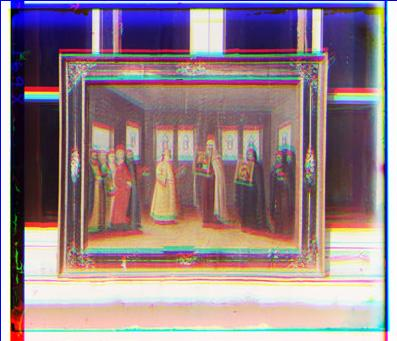
\includegraphics[scale=0.6]{processed/processed-128-00149v.jpg}~
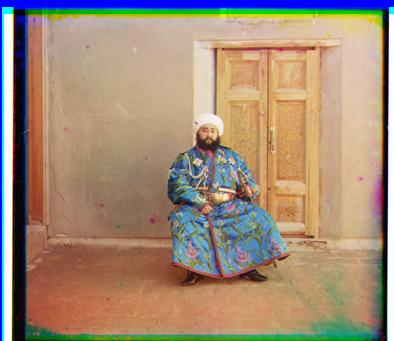
\includegraphics[scale=0.6]{processed/processed-128-00153v.jpg}
\end{center}

\begin{center}
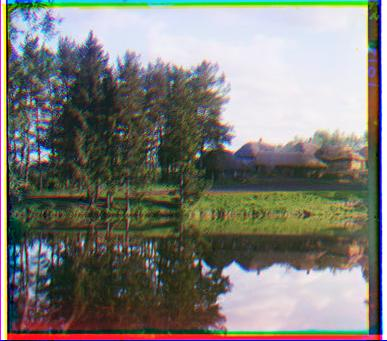
\includegraphics[scale=0.6]{processed/processed-128-00163v.jpg}~
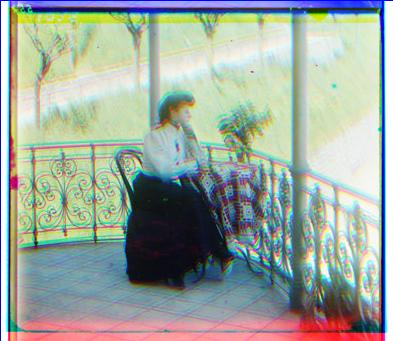
\includegraphics[scale=0.6]{processed/processed-128-00194v.jpg}
\end{center}

\begin{center}
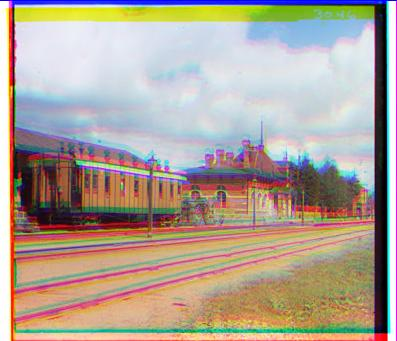
\includegraphics[scale=0.6]{processed/processed-128-00398v.jpg}~
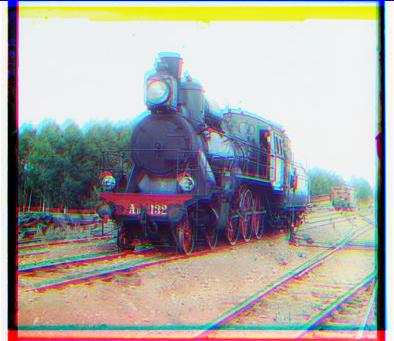
\includegraphics[scale=0.6]{processed/processed-128-00458v.jpg}
\end{center}

\begin{center}
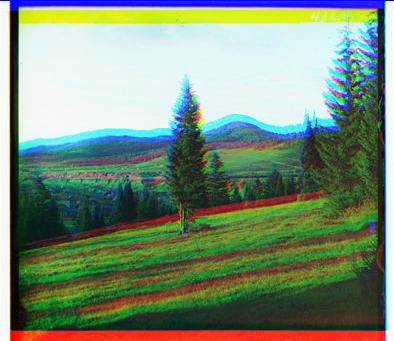
\includegraphics[scale=0.6]{processed/processed-128-00600v.jpg}~
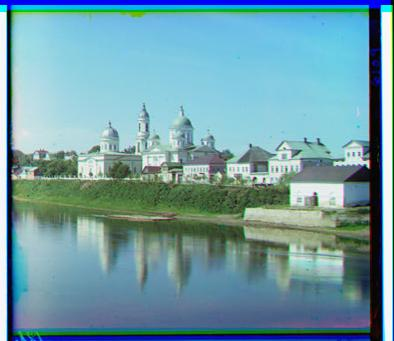
\includegraphics[scale=0.6]{processed/processed-128-01167v.jpg}
\end{center}

I found that the method worked well on most of the images, most of them looking just as aligned using 16 bins as with 128, with the exception of the single-tree image. This means that the coarse histogram often provided enough information about the image to align it without requiring futher binning, which makes sense since we were only shifting the image by 15 pixels anyway.

When I shifted the image, I padded with zeroes, which is the cause for the colorful edges -- a shifted layer with some white padding will allow other colos to show through.

I'm not sure why the tree image performed poorly compared to the others.
\end{document}